\subsection{Approaching Attribute Analysis}

Although each user account is associated with 33 publicly available attributes, only a few of these were of any interest for our purposes.  10 of the attributes are profile display settings, which were not considered.  Another 6 are user identifiers such as name and ID and are not of any use to network-level analysis.  We initially identified 14 potential attributes of interest.  Further description of these attributes is available in appendix \ref{app:user-attributes}.

After selecting attributes for consideration, we identified appropriate groupings for each attribute.  The format of the considered attributes took one of three forms.  These formats informed the manner in which they were grouped.  Many of the attributes had a finite number of options, such as a boolean value for \textit{Protected} or one of seven options for \textit{Language}.  A group was assigned for each possible value of these attributes.

The next field format was that of a continuous integer range, such as \textit{Follower Count} or \textit{Status Count}.  For these, groups took the form of a range of values.  It was important to create groups in such a manner that rare, high values user were clearly visible in the results.  It was also important that the large population of low value users were represented.  To accomplished this, we increased the range of our groupings logarithmically.

The final and most challenging format took the form a free text field.  Free text fields are used by the \textit{Bio}, \textit{URL} and \textit{Location} attributes.  Of these, only \textit{Location} was considered in our study.  After parsing this field for identifiable locations  on a variety of scales, it was decided that groupings by U.S. state would be the most impactful.  Of these, results for the top ten most popular states are included in this paper.

Paragraph: Mention the simple random survey of records that was performed, the percentage of users with no entry, the percentage of users with an indecipherable entry, etc.

After identifying discrete groupings for each attribute it became possible to enumerate all possible attribute relationships within our dataset.  Each edge in our subgraph represents a relationship between two Twitter users, each with a group assignment for each attribute.  We created a unique identifier for all possible relationships for each attribute.  We then processed our dataset by assigning these identifiers and counting their frequency.

\begin{figure*}[t]
 \centering
 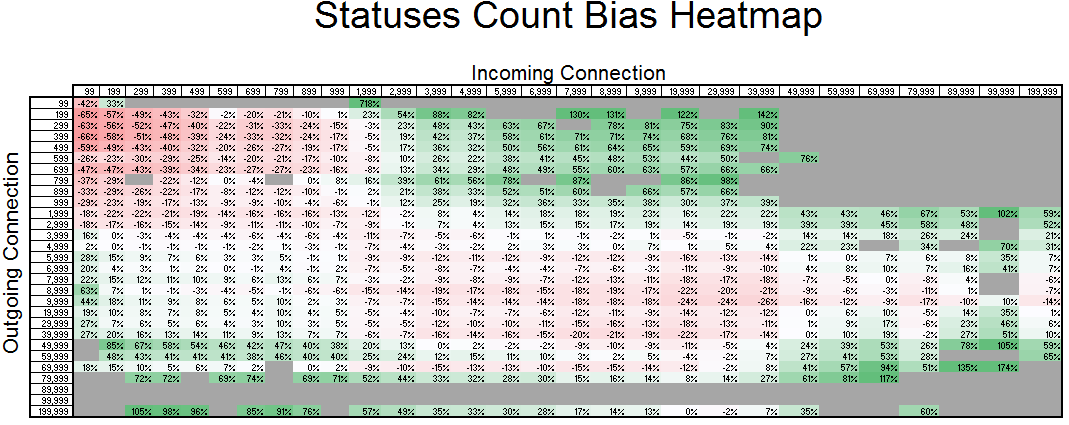
\includegraphics[bb=0 0 802 319,scale=.53]{./images/statuses_count.png}
 % statuses_count.png: 1069x425 pixel, 96dpi, 28.29x11.25 cm, bb=0 0 802 319
 \label{fig:status_count}
 \caption{A connectivity bias chart for number of status updates in logarithmically increasing groupings.}
\end{figure*}

\begin{figure*}[t]
 \centering
 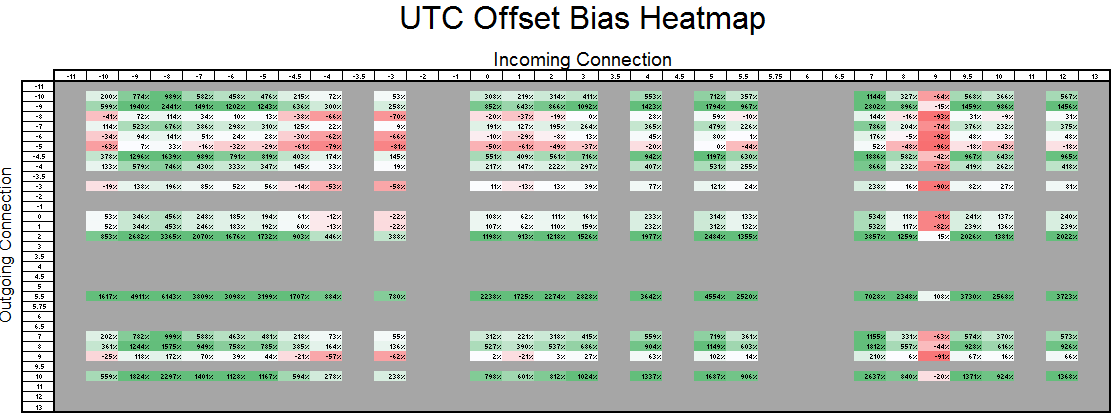
\includegraphics[bb=0 0 840 315,scale=.5]{./images/utc_offset.png}
 % utc_offset.png: 1120x420 pixel, 96dpi, 29.64x11.11 cm, bb=0 0 840 315
 \caption{A connectivity bias chart for Coordinated Universal Time (UTC) offset.}
 \label{fig:utc_offset}
\end{figure*}

\subsection{Measuring Bias}

Through data processing we obtained a set of values $A_{XY}$, representing the actual count of each possible attribute relationship \textit{X follows Y}.  However, this value alone is insufficient for measuring network bias.  It does not consider the frequency of users of attribute $X$ or $Y$.  It also does not consider the total number of outgoing edges from $X$, $X_{out}$ ,or incoming edges to $Y$, $Y_{in}$.  Before network bias can be determined it is necessary to normalize $A_{XY}$ against the value one would expect in a randomized, bias-free version of the graph.  This value is given by:

\[R_{XY} = \frac{X_{out}*Y_{in}}{\sum_{x,y,z}u}\]

where $X_{out}$ is the number of outgoing edges from $X$, $Y_{out}$ is the number of incoming edges to $Y$, and $\sum_{x,y,z}u$ is the sum of all edges for all attribute values in the network.  For our Twitter network, $R_{XY}$ is consistent when considered from both the incoming and outgoing edge perspective because of following fact:

\[\sum_{x,y,z}u_{out} = \sum_{x,y,z}u_{in}\]

Given $A_{XY}$ and $R_{XY}$, the bias for the relationship \textit{X follows Y} is given by:

\[B_{XY}=\frac{A_{XY}-R_{XY}}{R_{XY}}\]

A positive $B_{XY}$ indicates that group $X$ is biased towards following group $Y$.  A negative $B_{XY}$ indicates that group $X$ is biased against following group $Y$.  If $[B_{XY}]$ is very nearly zero, no bias is observed.  If $[B_{XY}] > 1$ then the relationship \textit{X follows Y} is biased to the point that it is several times more frequent or infrequent than would be expected in a randomized graph.
